\chapter{Literature Review}
\label{ch:literature_review}

This chapter presents the literature review of this study. First, it highlights key characteristics—unique features, strong points, and downsides—of some existing implementations. It then summarises the advantages and drawbacks of the two main types of persistence: state-based and change-based persistence, and it introduces desirable characteristics for a new change-based persistence implementation. This chapter then reviews the related work on identifying differences and detecting conflicts between versions of models. It then presents the challenges that model differencing and conflict detection are currently dealing with, as well as the downsides of existing approaches to solving the problems, which gives motivation to this research to come up with a new solution. Last, the conclusions of the literature review are presented.

\section{Models in This Research}
\label{sec:models_in_this_research)}

A model is an abstract representation of an entity \cite{volter2013model}. It can be used for different purposes: as a sketch to communicate a system, as a blueprint to define the specification of a system, or as a modifiable artefact to generate a working system \cite{fowler2019umlmode}. In model-based software engineering, the latter is the scenario in which models are mainly used.
In that scenario, a model is created using a modelling language, and the model should conform to its meta-model—an abstraction that describes the model. Later, the model can be transformed to generate a software artefact through model transformation/code generation \cite{brambilla2012model}. The software artefact, its model, and the model’s meta-model create a three-layered abstraction which is known as the three-layer meta-modelling architecture.

Eclipse Modeling Framework (EMF) \cite{steinberg2008emf} is a technical implementation of such an architecture. It is a framework and code-generating facility that allows developers to define meta-models, create models, and generate implementations of the models \cite{steinberg2008emf}. In this research and literature review, we focus on models and modelling tools that support the three-layer meta-modelling architecture of EMF.

\section{Model Persistence}
\label{sec:model_persistence}
In constructing models, modelling tools should be able to support model persistence so that models under construction can be saved at any time and reloaded for further modification. Most tools persist models in a state-based format. That is, they capture a snapshot of a model at a time and then persist its entire state into storage. The model state can be persisted in different forms, such as text files, relational databases, or NoSQL databases.

\subsection{Text Files}
\label{sec:text_file}
The simplest and most common way to save a model is to persist it into a text file. By default, modelling tools that support the three-layer meta-modelling architectures of Eclipse Modeling Framework (EMF) \cite{steinberg2008emf} persist a model in a text file with a format of Metadata Interchange (XMI)—a standard issued by Object Management Group (OMG) for exchanging metadata information using Extensible Markup Language (XML) \cite{omg2018xmi}.

Since it is the default for persisting EMF models, it is supported by most modelling tools. To modify a model persisted in an XMI file, such as performing create, read, update, delete (CRUD) operations, a tool has to de-serialise and load the model from the file into memory. This can be a problem when we want to make a few changes but the size of the model is very large—it takes considerable time and memory to load the model. Also, when it is saved, the model must be persisted in its entirety. This is not efficient when we made only a few changes. Since it is a text-based file, the model can be duplicated and shared with minimum effort, e.g. through manual copy or version control systems (e.g. Git \cite{git2019about} and SVN \cite{apache2019svn}). However, for model differencing (see Section \ref{sec:model_differencing_and_conflict_detection}), text-based differencing \cite{DBLP:journals/algorithmica/Meyers86} cannot be applied accurately to XMI files since they are essentially tree documents which require different differencing approaches \cite{wang2003xdiff}.

\subsection{Relational Databases}
\label{sec:relational_databases}
Models can also be persisted into relational databases. EMF Teneo \cite{eclipse2017teneo} is a solution that integrates EMF with existing persistency solutions, such as Hibernate \cite{hibernate2019hibernateorm} and EclipseLink \cite{eclipse2019eclipselink}. Thus, it can persist EMF models into relational database backends. In this way, EMF Teneo can utilise the power of storage, caching, and querying of the database backends. It also supports the automatic mapping of models to relational model schema with flexible mapping customisation. Using relational databases as its backends enables EMF Teneo to support the lazy loading of models. So, when performing CRUD operations, it only loads and saves relevant elements and features—not the entire model—into and from memory. This is efficient in terms of memory usage.

Similar to EMF Teneo, Connected Data Objects (CDO) \cite{eclipse2019cdo} also supports persisting models into various database elements model persistence (e.g. relational and NoSQL databases). It is a development-time model and meta-model repository as well as a distribution and runtime persistence framework for EMF-based application systems. It supports model versioning and can perform model differencing and conflict detection—it uses EMF Compare \cite{emfcompare2018developer} to perform the comparison \cite{cdo2019emfcompare}. One downside of CDO is that it requires the use of a separate version control system (e.g. a Git repository for code and a CDO repository for models). This can introduce fragmentation and create challenges to file administration \cite{barmpis2014evaluation}.

\subsection{NoSQL Databases}
\label{sec:NoSQL Databases}
In the era where data are abundant and models are getting larger, the ability to handle large models is necessary. Tools, such as Morsa \cite{DBLP:conf/models/Espinazo-PaganCM11} and NeoEMF \cite{daniel2016neoemf}, have been developed to persist models into non-relational (NoSQL) databases. Morsa saves models in documents with MongoDB as its backend \cite{mongodb}, while NeoEMF persists models in multiple NoSQL backends: Neo4j \cite{neo4j2019neo4j} for Graphs, MapDB \cite{mapdb2019mapdb} for Maps, and Apache HBase \cite{apache2019hbase} for Column datastores. The advantages of using NoSQL databases are that users are given options to choose which datastores—with some degree for configuration—that best fit the characteristics of their models and meta-models. This helps to maximise the features the backends provide, such as lazy loading and caching. Neither Morsa nor NeoEMF provides built-in support for versioning, and models are eventually stored in binary files/folders which are known to be a poor fit for text-oriented version control systems like Git and SVN.

\subsection{Change-based Representation (EMF Store)}
\label{sec:change_based_representation}
All the solutions previously mentioned persist models in state-based formats. EMF Store \cite{koegel2010emfstore} takes a different approach; it persists models in a change-based representation. EMF Store appears to be the only current implementation of change-based persistence for EMF models.

EMF Store is a model repository, and it supports collaborative editing and versioning of models \cite{emfstore2019what}. Instead of using standard text-oriented version controls (e.g., Git, SVN) for model versioning, EMF Store has its own dedicated, change-based, model-oriented versioning mechanism. Models are shared through a server and distributed to client applications. Clients can modify the models in parallel, offline or online, and synchronise with the server. Conflicts caused by concurrent modification are detected automatically, and they can be resolved interactively by users. The historical changes to models are kept on the server, and different versions of a model as well as changes that produced them can be retrieved from the server.

In EMF Store, to version models, a project must first be created. A project can contain one or more models. Every project has a version history, and each version represents a commit of a client. A commit sends a package of changes to the server. The package itself contains a collection of operations that transforms the project to a newer version or can be expressed as the differences (the deltas) between the two versions. An operation can be add, delete, set, unset, or move that modifies an element or feature, or it can be a composite operation—one that consists of many operations, e.g. re-factoring, which moves a method to a superclass.

To obtain a specific version of an existing project, a client performs a checkout. This version is called the base version on the client side. The client can then modify this version. Every operation applied to the version is recorded by EMF Store. When the client commits, these operations are put into one package and sent to the server. If the base version is still the head version of the project on the server, the commit is accepted, and a new version is created. If the base version is not the head version, it means that another client has committed its changes to the server. Thus, the current client has to synchronise it by updating its local project. This is the state where conflicts can happen between the incoming version and local changes, that is, when they modify the same element or feature of a model. EMF Store performs conflict detection to identify conflicts automatically. The mechanism of EMF Store to identify conflicts is discussed in detail in Section \ref{sec:emfstore_conflict_detection}.

As an illustration to show how EMF Store works, let's say that Jane's created a project on the server (Figure \ref{fig:emfstore_example}, step 1) setting an initial version, \textsf{v0}, of the model. She also shared it so that her team members could also work on the same project. Jane then created an initial model (step 2) and committed it to the server (step 3). As she committed her work on the server, operations \textsf{o1} and \textsf{o2} recorded while she was creating the initial model were also sent to the server producing version \textsf{v1}.

\begin{figure*}[h]
  \centering
  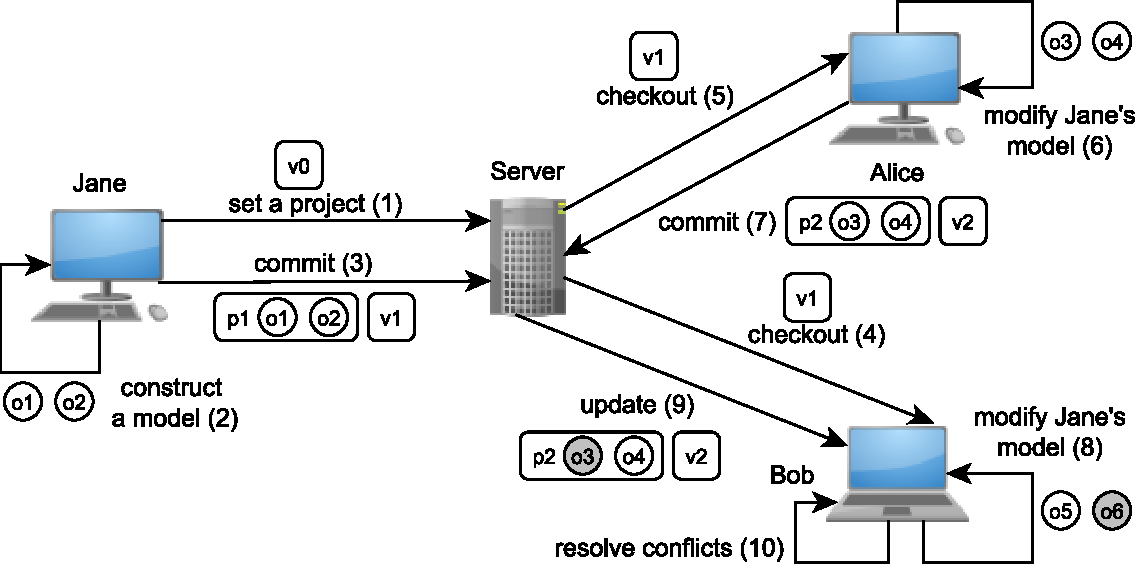
\includegraphics[width=\linewidth]{emfstore_example}
  \caption{An example to show how EMF Store works.}
  \label{fig:emfstore_example}
\end{figure*}

Bob and Alice then checked out Jane's work from then server creating copies of version \textsf{v1} on their local machines (steps 4 and 5).  Alice edited Jane's model by performing operations \textsf{o3} and \textsf{04} (step 6). She then committed her to the server, producing version \textsf{v2} (steps 7). Her commit was straightforward since her base version \textsf{v1} was the same as on the server --- no conflict detection is needed. After the commit, the server hold three versions of the model, \textsf{v0}, \textsf{v1}, and \textsf{v2}, including with their packages of operations, \textsf{p1}, containing \textsf{o1} and \textsf{o2}, and \textsf{p2}, containing \textsf{o3} and \textsf{o4}.

Bob also modified Jane's model in parallel. He performed operations \textsf{o5} and \textsf{o6} (step 8). However, when he tried to commit his work, he was required to update his work (step 9) since his base version was different from the one that was on the server due to the previous commit performed by Alice. His base version was \textsf{v1}, while \textsf{v2} was the latest version on the server. When updating, a conflict detection was performed to detect conflicts between the server's operations and his local operations. If there was a conflict, he was required to solve the conflict first before he could commit his work to the server (step 10).

\begin{table*}[]
  \centering
  \caption{Advantages and downsides of different model persistence solutions.}
  \label{table:model_persistence_comparison}
  \begin{scriptsize}
    \begin{tabular}{
        |>{\centering\arraybackslash}m{0.1\linewidth}
        |>{\centering\arraybackslash}m{0.4\linewidth}
        |>{\centering\arraybackslash}m{0.4\linewidth}
        |}
      \hline
      \textbf{Product} & \textbf{Advantages} & \textbf{Downsides} \\
      \hline
      XMI
      &
      \begin{minipage}[t]{\linewidth}
        \raggedright
        \begin{itemize}[leftmargin=7pt]
          \setlength
          \item[+] default standard, widely supported
          \item[+] easy to duplicate and share by manual copy or text-oriented version controls
          \item[]
        \end{itemize}
      \end{minipage}
      &
      \begin{minipage}[t]{\linewidth}
        \raggedright
        \begin{itemize}[leftmargin=5pt]
          \setlength
          \item[--] requires loading the entire model to modify
          \item[--] a model is saved in its entirety
          \item[--] supports text-oriented version controls, but applying text-based differencing might produce inaccurate results
          \item[]
        \end{itemize}
      \end{minipage}
      \\
      \hline
      Teneo
      &
      \begin{minipage}[t]{\linewidth}
        \raggedright
        \begin{itemize}[leftmargin=7pt]
          \setlength
          \item[+] supports lazy loading, only load and save affected elements and features when performing CRUD operations
          \item[+] can be supported by database backends: rollback, caching, etc.
          \item[]
        \end{itemize}
      \end{minipage}
      &
      \begin{minipage}[t]{\linewidth}
        \raggedright
        \begin{itemize}[leftmargin=7pt]
          \setlength
          \item[--] does not support model versioning, comparison, and merging
          \item[--] multiple concurrent accesses can cause a bottleneck
          % \item[--] performance on loading and saving for CRUD operations depends on the database backend
          \item[--] poor fit for text-oriented version controls since models are persisted in database
          \item[]
        \end{itemize}
      \end{minipage}
      \\
      \hline
      CDO
      &
      \begin{minipage}[t]{\linewidth}
        \raggedright
        \begin{itemize}[leftmargin=7pt]
          \setlength
          \item[+] supports lazy loading, only load and save affected elements and features when performing CRUD operations
          \item[+] supports model versioning, comparison, and merging
          \item[+] can be supported by database backends: rollback, caching, etc.
          \item[]
        \end{itemize}
      \end{minipage}
      &
      \begin{minipage}[t]{\linewidth}
        \raggedright
        \begin{itemize}[leftmargin=7pt]
          \setlength
          % \item[--] performance on loading and saving for CRUD operations depends on the database backend
          \item[--] fragmentation and administration challenges because of separation of version controls between models and code
          \item[--] poor fit for text-oriented version controls since models are persisted in database
          \item[]
        \end{itemize}
      \end{minipage}
      \\
      \hline
      Morsa \& NeoEMF
      &
      \begin{minipage}[t]{\linewidth}
        \raggedright
        \vspace{-12pt}
        \begin{itemize}[leftmargin=7pt]
          \setlength
          \item[+] supports lazy loading, only load and save affected elements and features when performing CRUD operations
          \item[+] can be supported by NoSQL backends: handling big data, graph data, etc.
          \item[]
        \end{itemize}
      \end{minipage}
      &
      \begin{minipage}[t]{\linewidth}
        \raggedright
        \vspace{-12pt}
        \begin{itemize}[leftmargin=7pt]
          \setlength
          \item[--] do not support model versioning, comparison, and merging
          % \item[--] performance on loading and saving for CRUD operations depends on the database backend
          \item[--] poor fit for text-oriented version controls since models are persisted in database
          \item[]
        \end{itemize}
      \end{minipage}
      \\
      \hline
      EMF Store
      &
      \begin{minipage}[t]{\linewidth}
        \raggedright
        \vspace{-12pt}
        \begin{itemize}[leftmargin=7pt]
          \setlength
          \item[+] supports semantic versioning of models, which allows model merging and conflict detection to be more effective
          \item[+] faster in detecting conflicts when numbers of changes are relatively small
          \item[]
        \end{itemize}
      \end{minipage}
      &
      \begin{minipage}[t]{\linewidth}
        \raggedright
        \vspace{-12pt}
        \begin{itemize}[leftmargin=7pt]
          \setlength
          \item[--] requires loading the entire model to modify
          \item[--] a model is saved in its entirety even for small changes
          \item[--] persists models in the forms of files/folders and using its own mechanism for model versioning; thus, it is a poor fit for text-oriented version controls
          \item[]
        \end{itemize}
      \end{minipage}
      \\
      \hline
    \end{tabular}
  \end{scriptsize}
\end{table*}

The primary motivation from EMF Store to a change-based approach is that calculating the differences between two versions in state-based persistence can be expensive and less accurate \cite{emfstore2019versioning} (State-based model differencing identifies differences using LCS algorithms \cite{emfcompare2018developer,DBLP:journals/algorithmica/Meyers86}, not the real changes). Since it follows a change-based approach, EMF Store does not store the state of every version. It saves operations of each version in an ordered manner only so they can be executed and reversed to obtain the states between versions. Nevertheless, it also stores the intermediate cached states for selected versions, including the head version, to speed up the retrieval of specific versions.

The advantages of EMF Store are that it was designed to allow semantic versioning of models. It can make model differencing and conflict detection more accurate and efficient rather than they are on state-based model persistence \cite{emfstore2019versioning}. By default, the packages of operations are persisted in XMI files, but EMF Store can also be configured to use other backends like MongoDB \cite{emfstore2019mongodb}. The downsides of EMF Store are that it has its own mechanism for controlling versions. This limits its adopters to use common text-oriented version controls \cite{emfstore2019getting}, such as Git and SVN. Its performance can also degrade as more models/users are added to a repository \cite{KolovosRMPGCLRV13}.

The advantages and downsides of the different model persistence solutions presented in this section can be found in Table \ref{table:model_persistence_comparison}. These advantages and downsides reveal points to consider on how to design a change-based model persistence format that is compatible with version control systems such as Git and SVN. These considerations are presented in Section \ref{sec:a_new_change_based_persistence}.

\subsection{Change-based vs. State-based Persistence}
\label{sec:change_based_vs_state_based_persistence}
This section compares the advantages and drawbacks of change-based and state-based persistence in general, not limited to EMF models. Change-based persistence works by persisting the complete change history of an artefact instead of persisting a snapshot—the entire state—of an artefact at a time. The concept of change-based persistence is not new; it has been used to persist changes of software, object-oriented databases, hierarchical documents, and models \cite{DBLP:journals/entcs/RobbesL07,DBLP:conf/sde/LippeO92,DBLP:conf/caise/IgnatN05,koegel2010emfstore}.

Change-based persistence offers two main advantages. First, it records information (e.g. types of changes, the order of the changes, elements that were changed, and previous values) with finer granularity. This can improve the accuracy of change detection \cite{DBLP:journals/entcs/RobbesL07,DBLP:conf/sde/LippeO92,DBLP:conf/caise/IgnatN05,mens2002state}. Second, it records changes in an ordered manner, which means that changes made to an artefact can be identified sequentially without having to explore and compare all elements of compared versions of an artefact \cite{DBLP:conf/edoc/KoegelHLHD10}. The advantages to detect changes more precisely and much faster can then have related benefits: (1) developers can compare and merge artefacts in collaborative environments \cite{DBLP:conf/sde/LippeO92,DBLP:conf/caise/IgnatN05,koegel2010emfstore} and (2) incremental management \cite{jouault2010towards,DBLP:conf/ecmdafa/OgunyomiRK15, DBLP:conf/ecmdafa/RathHV12}. Moreover, changed-based persistence contains a wealth of information which can be exploited for analytics \cite{DBLP:journals/entcs/RobbesL07}.

Nevertheless, change-based persistence also comes with downsides, such as ever-growing artefact files \cite{DBLP:journals/entcs/RobbesL07,DBLP:conf/edoc/KoegelHLHD10} and increased artefact loading time \cite{mens2002state}, which increases storage and computation costs. An artefact that is frequently modified will increase considerably in file size since every change is added to the file. The increased file size (proportional to the number of persisted changes) will, in turn, increase the loading time of the artefact since all changes must be replayed to reconstruct the artefact’s eventual state.

%These downsides must be mitigated to enable the practical adoption of change-based persistence.
%One approach to reducing the file size of change-based models is to remove changes that do not affect the eventual
%state of the model. For increased loading time, it can be mitigated by ignoring—i.e. not replaying—changes
%that are cancelled out by later changes or by employing change-based and state-based persistence side-by-side so that the
%benefits of state-based persistence on loading time can be obtained.

Other downsides are that change-based persistence requires
integration with existing tools—since it is still a non-standard approach—for its adoption \cite{koegel2010emfstore},
and it still has limited support for standard, text-based version controls for collaborative development \cite{koegel2010emfstore}.
These downsides can be addressed by developing a change-based persistence plugin for a specific development environment
(e.g. Eclipse) and persisting changes in text-based format to support text-based version controls (e.g. Git, SVN).

In summary, state-based persistence has several strong points. First, since it is the default standard persistence approach for most artefacts, it requires minimum effort to integrate with existing tools \cite{koegel2010emfstore}. Second, it is faster in loading artefacts persisted in state-based format since there is no need to replay all changes as with change-based persistence. Also, some artefacts support lazy loading. For example, an artefact is not loaded in its entirety upfront. Only parts affected by an operation are loaded into memory. This enables faster CRUD (create, read, update, delete) operations \cite{DBLP:conf/models/Espinazo-PaganCM11,daniel2016neoemf}.

\begin{table*}[h]
  \centering
  \caption{The advantages and downsides of change-based and state-based persistence.}
  \label{table:advantages_drawbacks}
  \begin{scriptsize}
    \begin{tabular}
      {|>{\centering\arraybackslash}p{1.1cm}|>{\centering\arraybackslash}p{1.1cm}|>{\centering\arraybackslash}p{5cm}|>{\centering\arraybackslash}p{5cm}|}
      \hline
      \multicolumn{2}{|c|}{\textbf{Dimension}}&\textbf{Change-based Approach}&\textbf{State-based Approach}\\
      \hline
      \multicolumn{2}{|p{2.2cm}|}{\centering Advantages} &
      \begin{minipage}[t]{5cm}
        \begin{itemize}[leftmargin=9pt]
          \setlength\itemsep{2pt}
          \item[+] More accurate, carries semantic information \cite{DBLP:journals/entcs/RobbesL07,DBLP:conf/sde/LippeO92,DBLP:conf/caise/IgnatN05,mens2002state}
          \item[+] Faster and more accurate for detecting changes, comparison, and merging \cite{DBLP:conf/sde/LippeO92,DBLP:conf/caise/IgnatN05,koegel2010emfstore}
          \item[+] Information carried is useful for analytics \cite{DBLP:journals/entcs/RobbesL07}
        \end{itemize}
      \end{minipage}
      &
      \begin{minipage}[t]{5cm}
        \raggedright
        \begin{itemize}[leftmargin=9pt]
          \setlength\itemsep{2pt}
          \item[+] Faster for loading large artefacts \cite{DBLP:conf/models/Espinazo-PaganCM11,daniel2016neoemf,eclipse2019cdo}
          \item[+] A default standard, no need to integrate with existing tools \cite{koegel2010emfstore}
        \end{itemize}
      \end{minipage}
      \\
      \hline
      \multicolumn{2}{|p{2.2cm}|}{\centering Disadvantages} & \begin{minipage}[t]{5cm}
        \raggedright
        \begin{itemize}[leftmargin=9pt]
          \setlength\itemsep{2pt}
          \item[--] Increased record size \cite{DBLP:journals/entcs/RobbesL07,DBLP:conf/edoc/KoegelHLHD10}
          \item[--] Not efficient for replaying (loading) long records \cite{mens2002state}
          \item[--] Limited support from standard, text-based version controls (e.g. GitHub) \cite{koegel2010emfstore}
          \item[--] Not a standard, needs integration with existing tools \cite{koegel2010emfstore}
        \end{itemize}
      \end{minipage}
      &
      \begin{minipage}[t]{5cm}
        \raggedright
        \begin{itemize}[leftmargin=9pt]
          \setlength\itemsep{2pt}
          \item[--] Slower for saving changes (XMIs) \cite{mens2002state,daniel2016neoemf,DBLP:conf/models/Espinazo-PaganCM11}
          \item[--] Slower for comparison \cite{DBLP:conf/edoc/KoegelHLHD10}
          \item[--] Less accurate, does not carry semantic information \cite{mens2002state,DBLP:conf/edoc/KoegelHLHD10}
        \end{itemize}
      \end{minipage}
      \\
      \hline
    \end{tabular}
  \end{scriptsize}
\end{table*}

Compared to change-based persistence, state-based persistence also has downsides. First, it is slower than change-based persistence in saving changes \cite{mens2002state}. For an artefact persisted in state-based format and does not support lazy loading, the artefact must be persisted in its entirety even though only a single change has been made. Second, state-based persistence does not keep records of changes to an artefact. Thus, every part of the artefact must be checked for differences. This can be less efficient if the comparison is performed in a change-based format \cite{DBLP:conf/edoc/KoegelHLHD10}. Third, comparison in a state-based format requires identifying differences through a diffing process—not based on actual change records. So, it can be less accurate than a comparison in change-based persistence which is provided with more information to detect changes accurately \cite{mens2002state,DBLP:conf/edoc/KoegelHLHD10}. The advantages and downsides of change-based and state-based persistence are summarised in Table \ref{table:advantages_drawbacks}.

\section{Model Differencing and Conflict Detection}
\label{sec:model_differencing_and_conflict_detection} 
The history of model differencing and conflict detection can be traced back to the presence of the \textsf{diff} program on Unix or Unix-like platforms \cite{hunt1976algorithm}. Diffing is a function that compares text files ‘to determine how or whether they differ’ \cite{diff}. It is commonly known as the Longest Common Subsequence (LCS) algorithm \cite{bergroth2000lcs}, and it is equivalent to the Shortest Edit Script (SES) problem: finding the smallest number of edits (adds and deletes) to make a sequence equal to another sequence \cite{DBLP:journals/algorithmica/Meyers86}. LCS or SES algorithms are commonly implemented by Version Control Systems, such as SVN \cite{svn-diff} and Git \cite{git-diff}, in their \textsf{diff} programs to identify differences between versions of files.

Using diffing on graph-based artefacts, such as XML \cite{w3c-xml} and Ecore models \cite{steinberg2008emf}, is not straightforward since they are different from text files. For example, XML is a hierarchical document with a tree structure; one node can contain other nodes. The unique feature of XML is that its containment is unordered, whereas in text files differencing order is a necessary feature. This has been addressed by Wang et al. \cite{wang2003xdiff} by exploiting key XML structure characteristics. 

%% begin revision point 2
For example, in Listings \ref{lst:left_xml} and \ref{lst:right_xml}, we have two XML documents that are semantically equivalent. However, a text-based differencing will identify that `<c/>' is at different lines in both documents (at line 3 in the left document, at line 2 in the right document). Moreover, `<d/>' and `<d></d>' at line 4 are identified as two different lines even though they have the same meaning. This also applies to `<e></e>' that is expressed in two lines (lines 5, 6) in the left XML document but expressed as one line (line 5) in the right XML document.

\vspace{-20pt}
\begin{minipage}[t]{0.49\linewidth}
\begin{lstlisting}[style=eol,caption={Left XML document.}, label=lst:left_xml]
<a>
  <b/>
  <c/>
  <d/>
  <e>
  </e>
<a/>
\end{lstlisting}
\end{minipage}
\hfill
\begin{minipage}[t]{0.49\linewidth}
  \begin{lstlisting}[style=eol,caption={Right XML document.}, label=lst:right_xml]
<a>
  <c/>
  <b/>
  <d></d>
  <e></e>
<a/>
  \end{lstlisting}
\end{minipage}
%% end revision point 2

Identifying differences between Ecore models is even more complex than XML differencing since those models support multiple characteristics of features, such as attribute/reference, literal/object values, single/multiple values, and containment/non-containment\cite{steinberg2008emf}. There are several existing tools for model differencing. 

EMF Compare \cite{emfcompare2018developer} is a popular tool for comparing and merging EMF models, with generic support for different meta-models. It is an extensible framework, so it can be adapted to the specific needs of certain meta-models. EMF Compare works by matching elements of the models being compared and then executing differencing to identify the differences between them. Matching and differencing are discussed in detail in Chapter \ref{ch:model_differencing}. 

EMF DiffMerge (EDM) \cite{eclipse2019emfdiffmerge} is similar to EMF Compare except that its abstraction is at a lower level, and it is designed to prevent data loss and enforce model consistency \cite{eclipse2019emfdiffmerge2}. As a consequence, EMF Compare could use the EDM engine when it needs to enforce a particular consistency policy. Also, it supports scoping, which means that the comparison does not must be at the model level. It could also be applied to sets of model elements—subsets of models—that can be defined arbitrarily by using specific filters \cite{jaxenter2019emfdiffmerge}. In this study, EMF Compare is used as a baseline for evaluation because of its maturity and ongoing development activity. 

Other tools, such as SiDiff \cite{Treude2007SiDiff} and DSMDiff \cite{lin2009dsmdiff}, also provide language-agnostic graph-based model comparison, with some room for configuration (e.g., assigning different weights to features of types in the language). Additional expressive power—at the cost of increased complexity and configuration effort—is offered by dedicated comparison languages such as the Epsilon Comparison Language, which can be used to compare both homogeneous and heterogeneous models \cite{kolovos2009ecl}. All of these tools work with state-based persistence to identify differences between models.

Our literature review has not identified any other work that targets comparison of change-based models persisted in text files. Only EMF Store \cite{koegel2010emfstore} addresses change-based model conflict detection, but it persists models in its own dedicated backend system. Moreover, since it is designed to identify conflicts between changes, it does not give direct, summarised information about which parts of two versions of a model are different—not for model differencing. It only gives lists of changes to users. The summarised information is useful in the scenario where a model is excessively changed in both versions since users do not have to interpret the long lists to identify differences between the versions. Moreover, it works only on changes; it does not consider eventual states of models in detecting conflicts \cite{DBLP:conf/sfm/BroschKLSWW12}. Thus, if an element has been changed concurrently, but the changes produce eventual states that are equal to their original state, EMF Store still treats these changes as if they were in conflict. Database or dedicated-backend model persistence and version control solutions such as CDO \cite{eclipse2019cdo} and EMF Store provide model conflict detection capabilities between different versions of the same model, but they present integration challenges when users wish to use text-oriented version control systems (e.g. Git, SVN) which are typically file-based. Moreover, their performance can degrade as more models/users are added to a repository \cite{KolovosRMPGCLRV13}.

\subsection{The Challenges of Model Comparison}
\label{sec:the_key_challenge_of_incrementality}

Identifying differences between versions of models can become crucial for large evolving models, particularly in the later phases of the development cycle when many small changes are made to fine-tune the models \cite{selic2003pragmatics}. This challenge has been addressed by incremental model management where changes to models are recorded and used as the basis for effective incremental model processing operations. Egyed \cite{egyed2011automatically} has shown that the property-access recording approach is applicable to query such changes. More recent work has shown that variants of this approach can be used to achieve incrementality in a wide range of model processing operations, including model-to-model transformation \cite{jouault2010towards}, model-to-text transformation \cite{DBLP:conf/ecmdafa/OgunyomiRK15}, model validation, and pattern matching \cite{DBLP:conf/ecmdafa/RathHV12}—as long as the changes can be precisely identified.

Nonetheless, this approach works best at identifying differences between serial versions of a model; it is not as straightforward in identifying differences between parallel—branched—versions. In addition, the solutions in incremental model management are coupled with their execution engines. This means they work best in single-developer environments. (This is discussed further in Section \ref{sec:identifying_changes_in models}). In a collaborative setting, as the size and complexity of a model grows, it is common to manage the model in multiple parallel versions. Thus, the ability to identify differences between parallel versions and to detect conflicts between the differences is very important.

Model differencing and conflict detection must be executed before two versions of a model are merged. However, performing model differencing and conflict detection in the typical state-based approach is computationally expensive and memory-greedy. (This is discussed further in Section \ref{sec:identifying_changes_in models}). In traditional, state-based model comparison, every element of the versions being compared must be loaded into memory, matched, and then differenced \cite{emfcompare2018developer}. This is inefficient for large models that undergo only a few changes. A novel approach is required that can compare only elements that have been modified -- —not all elements—to speed up model comparison.

\subsection{Identifying Changes in Models}
\label{sec:identifying_changes_in models}
There are two approaches in the literature for identifying changes in models: using notification facilities and model differencing. These are reviewed inf the sections that follow.

\subsubsection{Notifications}
\label{sec:notifications}
In this approach, a model change tracking engine must hook into the notification facilities of the modelling tool used to edit the model, so that the engine can receive notifications as soon as a change happens (e.g. class \textsf{Giant} has been deleted, class \textsf{Character} has been renamed to ‘Hero’).
This is an approach taken by the IncQuery incremental pattern matching framework \cite{DBLP:conf/ecmdafa/RathHV12} and the ReactiveATL incremental model-to-model transformation engine \cite{DBLP:conf/ecmdafa/OgunyomiRK15}. The main advantage of this approach is that precise and fine-grained change notifications are provided for free by the modelling tool. (They do not need to be computed by the execution engine—which as discussed below can be expensive and inefficient).
On the downside, this approach is a poor fit for collaborative development settings where modelling and automated model processing activities are performed by different members of the team.

\subsubsection{Model Differencing}
\label{sec:model_differencing}
This approach eliminates the coupling between modelling tools and model change tracking engines. Instead of depending on live notifications, in this approach the developer needs to have access to a copy of the last or other version of the model, so it can be compared against the current version of the model (e.g. using a model-differencing framework such as EMF Compare\cite{emfcompare2018developer} or EMF DiffMerge \cite{eclipse2019emfdiffmerge}) and the differences (the delta) can be computed on demand. The main advantage of this approach is that it works well in a collaborative development environment where typically developers have distinct roles and responsibilities. On the downside, model comparison and differencing are computationally expensive and memory-greedy as both versions of the model must be loaded into memory before they can be compared.

In summary, tracking changes in models using notification facilities currently delivers significant performance benefits only in a single-developer environment as the approach is coupled to modelling tools.
As a result, in collaborative development environments, developers must either forgo the notification approach altogether or work with model differencing, which is computationally expensive and memory-greedy.

\section{Conclusions}
\label{sec:conclusions_2}
This chapter presented a review of literature in the areas of model persistence and differencing. It summarised the advantages and drawbacks of state-based and change-based model persistence, and related work on identifying differences and detecting conflicts between versions of models.
